\section{Techniques}

This section gives an overview of different techniques used in our crawler. We first show how we integrated a headless web browser into the harvesting process to support blogs that use JavaScript to display page content. The overall software architecture will then be discussed, introducing the Scrapy framework and the enrichments we implemented for our specific usage. Finally we will talk about the design choices we made in view of large scale deployment.


%%%%%%%%%%%%%%%%%%%%%%%%%%%%%%%%%
\subsection{JavaScript rendering}
% Introduction
JavaScript is a widely used language for client-side scripting. While some applications simply use it for aesthetics (menus, animations...), an increasing number of websites use JavaScript to download and display content. In such cases, traditional HTML based crawlers do not see web pages as they are presented to a human visitor and might therefore be obsolete for data extraction.

% Motivation
In our experiments whilst crawling the blog sphere, we encountered several blogs were data was missed because of the lack of JavaScript interpretation. The most frequent cases where blogs using the Disqus \cite{disqus2013} and LiveFyre \cite{livefyre2013} comment hosting services. For web-masters, these tools are very handy to setup because the entire comments infrastructure is externalized and the setup essentially comes down to including a JavaScript snippet in each target page. Both of these services heavily rely on JavaScript to download and display the comments, even providing functionalities such as real-time updates for edits and newly written comments. Less commonly, some blogs are fully rendered using JavaScript. When loading such websites, the web browser will not receive page contents as HTML files, but will instead have to execute JavaScript code to download and display page contents. The Blogger platform provides as a default template the \emph{Dynamic Views}, which uses this mechanism \cite{antinharasymiv2011}.

% The solution
To support blogs with JavaScript generated content, we embed a full web browser into the crawler. After considering multiple options, we opted for PhantomJS \cite{phantomjs2013}, a headless web browser with great performances and scripting capabilities. The JavaScript rendering is the very first step of web page processing. Therefore, Extracting blog post articles, comments or medias works equally well on blogs with JavaScript generated content and traditional HTML-only blogs.

% Click click scripting
When the number of comments on a page exceeds a certain threshold, both Disqus and LiveFyre will only load the most recent ones and the stream of comments will end with a \emph{Show More Comments} buttons. As part of the page loading process, we instruct PhantomJS to repeatedly click on these buttons until all comments are loaded. Paths to Disqus and LiveFyre \emph{Show More} buttons were manually obtained. They constitute the only non-generic element of our extraction stack which will require human intervention to maintain and extend to other commenting platforms.


%%%%%%%%%%%%%%%%%%%%%%%%%
\subsection{Architecture}

\begin{figure}
  \capstart
  \centering
  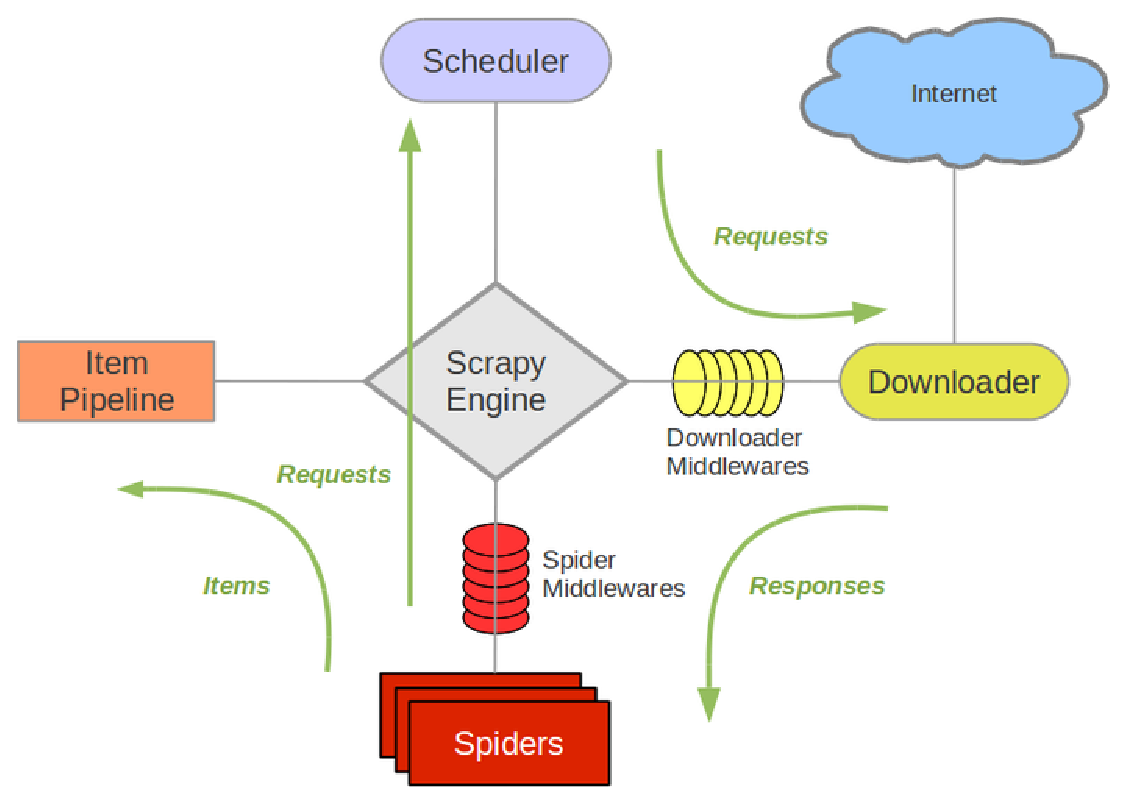
\includegraphics[width=0.47\textwidth]{scrapy_architecture}
  \caption{Overview of the crawler architecture.\\(Credit: Pablo Hoffman, Daniel Graña, \cite{scrapy2013})}
  \label{architecture}
\end{figure}

Our crawler is built on top of Scrapy \cite{scrapy2013}, an open source Python framework for web crawling. Scrapy provides an elegant and modular architecture illustrated in \autoref{architecture}. Several components can be plugged into Scrapy core infrastructure: \emph{Spiders}, \emph{Item Pipelines}, \emph{Downloader Middlewares} and \emph{Spider Middlewares}; each allowing us to implement a different type of functionalities.

Our use case has two types of spiders: \emph{NewCrawl} and \emph{UpdateCrawl}, which implement the logic to respectively crawl a new blog and get updates from a previously crawled blog. After being downloaded and identified as blog posts (details in \ref{enrichingscrapy}), pages are packed into \emph{Items} and sent through the following pipeline of operation:
\begin{enumerate}[noitemsep]
  \item Render JavaScript
  \item Extract content
  \item Extract comments
  \item Download media
  \item Propagate resulting records to the back end
\end{enumerate}
This pipeline design provides great modularity. Indeed, disabling JavaScript rendering or plugging in an alternative back-end can be done by editing one single line of code.


%%%%%%%%%%%%%%%%%%%%%%%%%%%%%
\subsection{Enriching Scrapy}\label{enrichingscrapy}
% into
In order to identify web pages as blog posts, our implementation enriches Scrapy with two components to narrow the extraction process to the subsets of blog pages holding blog posts: \emph{blog post identification} and \emph{download priority heuristic}.

% blog post identification
Given an entry point to a website, the default Scrapy behavior looks over all pages of the same domain in a \emph{last-in-first-out} manner. The \emph{blog post identification} function is able to identify from an URL whether or not the corresponding page is a blog post. Internally, for each blog, this function uses a regular expression constructed from web feed entry URLs. This simple approach requires that blogs use the same pattern for all posts (or false negative will occur) which has to be distinct for non-post pages (or false positive will occur). In practice, this assumption holds for all blog platforms we encountered and seems to be a common practice amongst web developers.

% download priority heuristic
In order to efficiently deal with blogs with a large number of non-blog-post pages, this \emph{blog post identification} mechanism is not sufficient. Indeed, after all pages identified as blog posts are processed, the crawler needs to download non-blog-post pages to search for additional blog posts. To replace the naive \emph{random walk}, \emph{depth first search} or \emph{breadth first search} web site traversals, we use a priority queue where priorities of new URLs are determined by a machine learning system. This mechanism has shown to be mandatory for blogs hosting on a single domain a large number of non-blog web pages, such as a forum or a wiki.

% Distance-Weighted k-Nearest-Neighbor
The idea is to give a high priority to URLs which are believed to point to pages with links to blog post. These predictions are done using an active \emph{Distance-Weighted k-Nearest-Neighbor} classifier \cite{dudani1976}. Let $L(u)$ be the number of links to blog posts contained in a page with URL $u$. Whenever a page is downloaded, it's URL $u$ and $L(u)$ are given to the machine learning system as training data. When the crawler encounters a new URL $v$, it will ask the machine learning system for a estimation of $L(v)$, and use this value as the download priority of $v$. $L(v)$ is estimated by doing a weighted average on the values of the $k$ URLs most similar to $v$.

%%%%%%%%%%%%%%%%%%%%%%%%
\subsection{Scalability}
When aiming to work with a large number of inputs, it is crucial to build every layer of a system with scalability in mind \cite{thereactivemanifesto2013}. The BlogForever crawler, and in particular the two core procedures \emph{NewCrawl} and \emph{UpdateCrawl}, are designed to be usable as part of an event-driven, scalable and fault resilient distributed system.

To go in this direction, we made the key design choice to have both \emph{NewCrawl} and \emph{UpdateCrawl} as stateless components. From a high level viewpoint, these two components are \emph{purely functional}:
%
\newcommand\URL{\mathbb{U}\text{RL}}
\newcommand\DATE{\mathbb{D}\text{ATE}}
\newcommand\RECORD{\mathbb{R}\text{ECORD}}
\begin{equation*}
  \begin{split}
    NewCrawl:    &~ \URL \rightarrow \mathcal{P}(\RECORD)\\
    UpdateCrawl: &~ \URL \times \DATE \rightarrow \mathcal{P}(\RECORD)
  \end{split}
\end{equation*}
%
Where $\URL$, $\DATE$ and $\RECORD$ are respectively the set of all URLs, dates and records, and $\mathcal{P}$ designates the powerset operator. By delegating all shared mutable state to the back end system (Invenio's database), web crawler instances can be added, removed, and used interchangeably.
